\section{ฟังก์ชันของการแปรผันที่มีขอบเขต}
ให้ $\Omega$ เป็นเซ็ตเปิดมีขอบเขตของ $ \mathbb{R}^{d}$ และให้ $u \in L^{1}(\Omega)$ กำหนดให้การแปรผันรวม $u$ เป็น

\begin{align} 
    \int_{\Omega} |Du| = \text{sup} \Big\{ \int_\Omega u \nabla \cdot \varphi \Big\}
\end{align}

เมื่อ  เป็น (Lebesgue measure) แลt $C_0^1 ( \Omega , \mathbb{R}^d)$ คือปริภูมิของฟังก์ชันต่อเนื่องที่หาอนุพันธ์ได้และกระชับใน $\Omega$

\hspace{1cm} ตามที่ได้ถูกกล่าวถึงใน \cite{ref:bounded_variation} สำหรับกรณีเฉพาะซึ่งเป็นที่น่าสนใจ $u \in C^1 (\Omega, \mathbb{R}^d )$ โดยการใช้ปริพันธ์แบบแยกส่วน

\begin{align}
    \int_\Omega u \nabla \cdot \varphi d x = - \int_\Omega \sum_{i=1}^{d} \frac{\partial u}{\partial x_i} \varphi_i d x
\end{align}

สำหรับทุก $\varphi \in C_0^1 (\Omega,\mathbb{R}^{d})^{d} $ และ

\begin{align}
    \int_\Omega | D u | = \int_\Omega | \nabla u | dx
\end{align}

ฟังก์ชัน $u \in L^1 (\Omega)$ เรียกว่ามีขอบเขตการแปรผันใน $\Omega$ ถ้า $\int_\Omega |Du| < \infty$ โดยเรากำหนดให้ $BV(\Omega)$ เป็นปริภูมิของฟังก์ชันทั้งหมดใน $L^1(\Omega)$ การแปรผันที่มีขอบเขต

\begin{Example}
    ฟังก์ชัน $f1, f2 \text{และ} f3 $ ต่อไปนี้กำหนดโดย
    \begin{align}
        f1(x) = sin x,
    \end{align}
    \begin{align}
        f2(x) = \left\{
            \begin{array}{ll}
              1/4, \hspace{1cm}  x \in [0,\Pi/8] \\
              1/2, \hspace{1cm}  x \in [\Pi/8,\Pi/4] \\
              3/4, \hspace{1cm}  x \in [\Pi/4,3\Pi/8] \\
              1, \hspace{1cm}  x \in [3\Pi/8,\Pi/2] \\
            \end{array}
          \right.
    \end{align}
    \begin{align}
        f3(x) = \frac{2x}{\Pi},
    \end{align}
    จาก $BV(\Omega)$ ซึ่ง $\Omega = [0, \Pi/2]$ และมีการแปรผันรวมมีค่าเป็น 1 ให้ฟังก์ชัน $f4$ กำหนดโดย
    \begin{align}
        f4(x) = \left\{ 
            \begin{array}{ll}
                0, \hspace{1cm}  x = 0 \\
                sin 1/x, \hspace{1cm} x \in (0,a) \text{และ} a > 0
            \end{array}
        \right.
    \end{align}
    
    มีการแปรผันไม่จำกัดและไม่อยู่ใน $BV(\Omega)$ ซึ่ง $\Omega = [0,a]$ สำหรับทุก $a > 0$
    \begin{figure}[H]
	\centering
	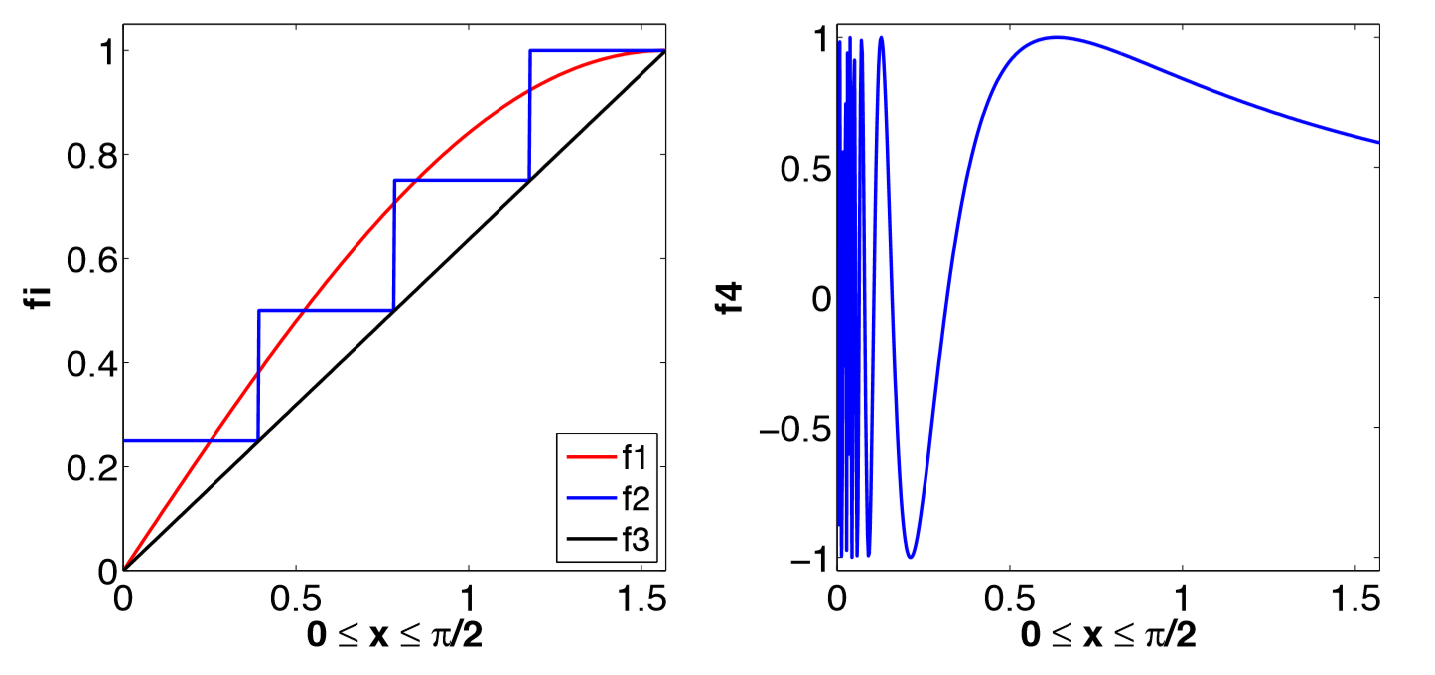
\includegraphics[width=0.8\linewidth]{image/boundary_condition/function_slove.png}
	\caption{ฟังก์ชันแปรผันมีขอบเขตทั้งสามฟังก์ชันที่มีการแปรผันรวมเหมือนกันเท่ากับ 1  และฟังก์ชันที่มีการแปรผันไม่จำกัด}
	\label{figure:sample-domain}
\end{figure}
\end{Example}

ซึ่งสำหรับในหัวข้อนี้เราสามารถสรุปได้เป็นสูตรของคลอเลีย (Coarea formula)

\begin{Theorem} (Coarea fomula) ให้ $\Omega \subset \mathbb{R}^d$ เป็นเซ็ตเปิดและให้ $ u \in BV(\Omega)$ และ $L_{\lambda} = \{ x \in \Omega | u(x) < \lambda \}$ เป็นระดับโดเมน (level domain) แล้ว
    \begin{align*}
        \int_{\Omega} | D u | = \int_{- \infty}^{\infty} Per(L_{\lambda}, \Omega) d \lambda
    \end{align*}
    เมื่อ $Per(L_{\lambda}, \Omega) = \int_{\Omega} |D_{x^{L_{\lambda}}}|$ คือ perimeter ของ $L_{\lambda}$ ใน $\Omega$ และ $\chi^{L_{\lambda}}$ คือลักษณะเฉพาะ (characteristic) ของฟังก์ชัน $L_{\lambda}$

    โดยบนพิสูจน์สามารถดูได้ใน \cite{ref:bounded_variation} 
\end{Theorem}